% !TEX program = xelatex
% !TEX root = report.tex
\documentclass[12pt,a4paper]{ctexart}

% ── packages ──
\usepackage[margin=2cm]{geometry}
\usepackage{graphicx}
\usepackage{booktabs}
\usepackage{hyperref}
\usepackage{xcolor}
\usepackage{enumitem}
\usepackage{tikz}
\usepackage{float}
\usepackage{caption}
\usepackage{array}
\usepackage{longtable}
\usetikzlibrary{arrows.meta,positioning}

\hypersetup{
  colorlinks=true,
  linkcolor=blue!60!black,
  urlcolor=blue!60!black,
  citecolor=blue!60!black,
}

\definecolor{passgreen}{RGB}{39,174,96}
\definecolor{headerbg}{RGB}{44,62,80}
\graphicspath{{picture/}{report_assets/}{../../report_assets/}}

\tikzset{
  fsmstate/.style={
    draw,
    rounded corners=2pt,
    align=center,
    inner sep=4pt,
    fill=gray!6,
    font=\small
  },
  alarmstate/.style={fsmstate, fill=red!8},
  timeoutstate/.style={fsmstate, fill=yellow!18},
  fsmedge/.style={->, thick, >=Latex},
  fsmlabel/.style={font=\small, fill=white, inner sep=1.5pt}
}

\newcommand{\PartOneFSM}{%
\resizebox{0.82\textwidth}{!}{%
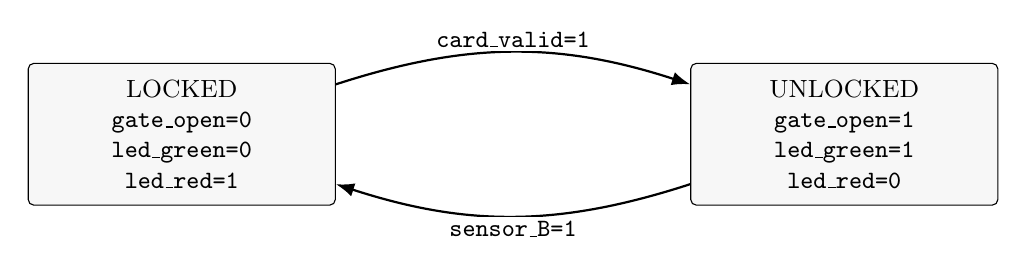
\begin{tikzpicture}
\node[fsmstate, minimum width=39mm, minimum height=18mm] (locked)
  {LOCKED\\\texttt{gate\_open=0}\\\texttt{led\_green=0}\\\texttt{led\_red=1}};
\node[fsmstate, minimum width=39mm, minimum height=18mm, right=45mm of locked] (unlocked)
  {UNLOCKED\\\texttt{gate\_open=1}\\\texttt{led\_green=1}\\\texttt{led\_red=0}};
\draw[fsmedge] (locked) to[bend left=18] node[fsmlabel, above] {\texttt{card\_valid=1}} (unlocked);
\draw[fsmedge] (unlocked) to[bend left=18] node[fsmlabel, below] {\texttt{sensor\_B=1}} (locked);
\end{tikzpicture}%
}}

\newcommand{\PartTwoFSM}{%
\resizebox{0.98\textwidth}{!}{%
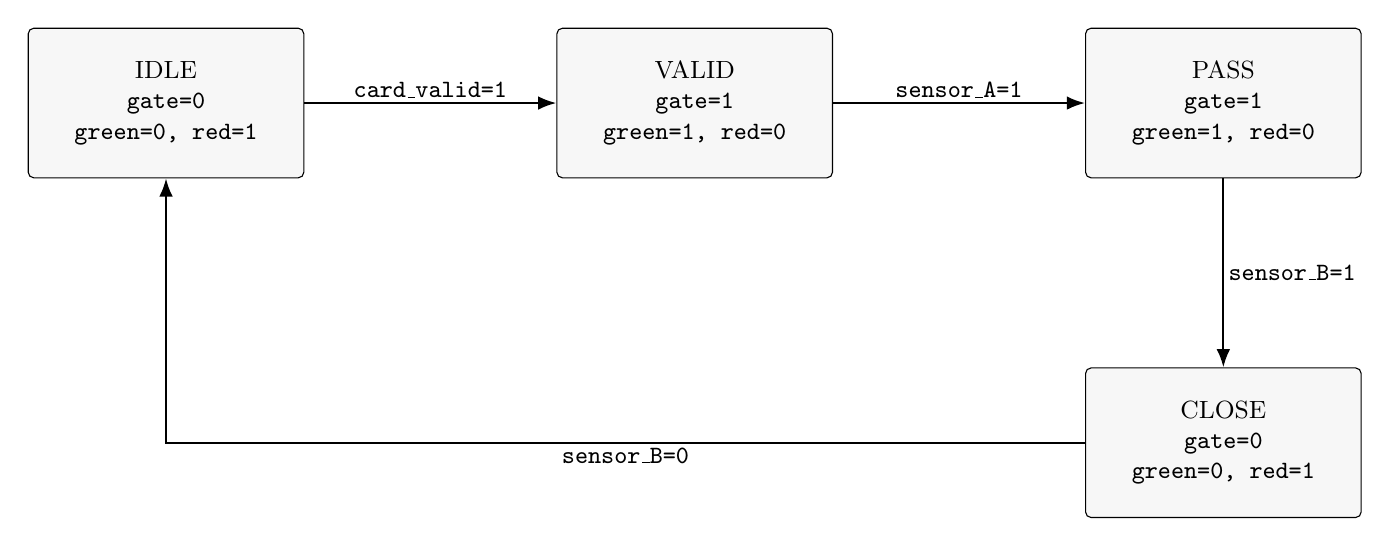
\begin{tikzpicture}
\node[fsmstate, minimum width=35mm, minimum height=19mm] (idle)
  {IDLE\\\texttt{gate=0}\\\texttt{green=0, red=1}};
\node[fsmstate, minimum width=35mm, minimum height=19mm, right=32mm of idle] (valid)
  {VALID\\\texttt{gate=1}\\\texttt{green=1, red=0}};
\node[fsmstate, minimum width=35mm, minimum height=19mm, right=32mm of valid] (pass)
  {PASS\\\texttt{gate=1}\\\texttt{green=1, red=0}};
\node[fsmstate, minimum width=35mm, minimum height=19mm, below=24mm of pass] (close)
  {CLOSE\\\texttt{gate=0}\\\texttt{green=0, red=1}};
\draw[fsmedge] (idle) -- node[fsmlabel, above] {\texttt{card\_valid=1}} (valid);
\draw[fsmedge] (valid) -- node[fsmlabel, above] {\texttt{sensor\_A=1}} (pass);
\draw[fsmedge] (pass) -- node[fsmlabel, right] {\texttt{sensor\_B=1}} (close);
\draw[fsmedge] (close.west) -| node[fsmlabel, near start, below] {\texttt{sensor\_B=0}} (idle.south);
\end{tikzpicture}%
}}

\newcommand{\PartThreeFSM}{%
\resizebox{\textwidth}{!}{%
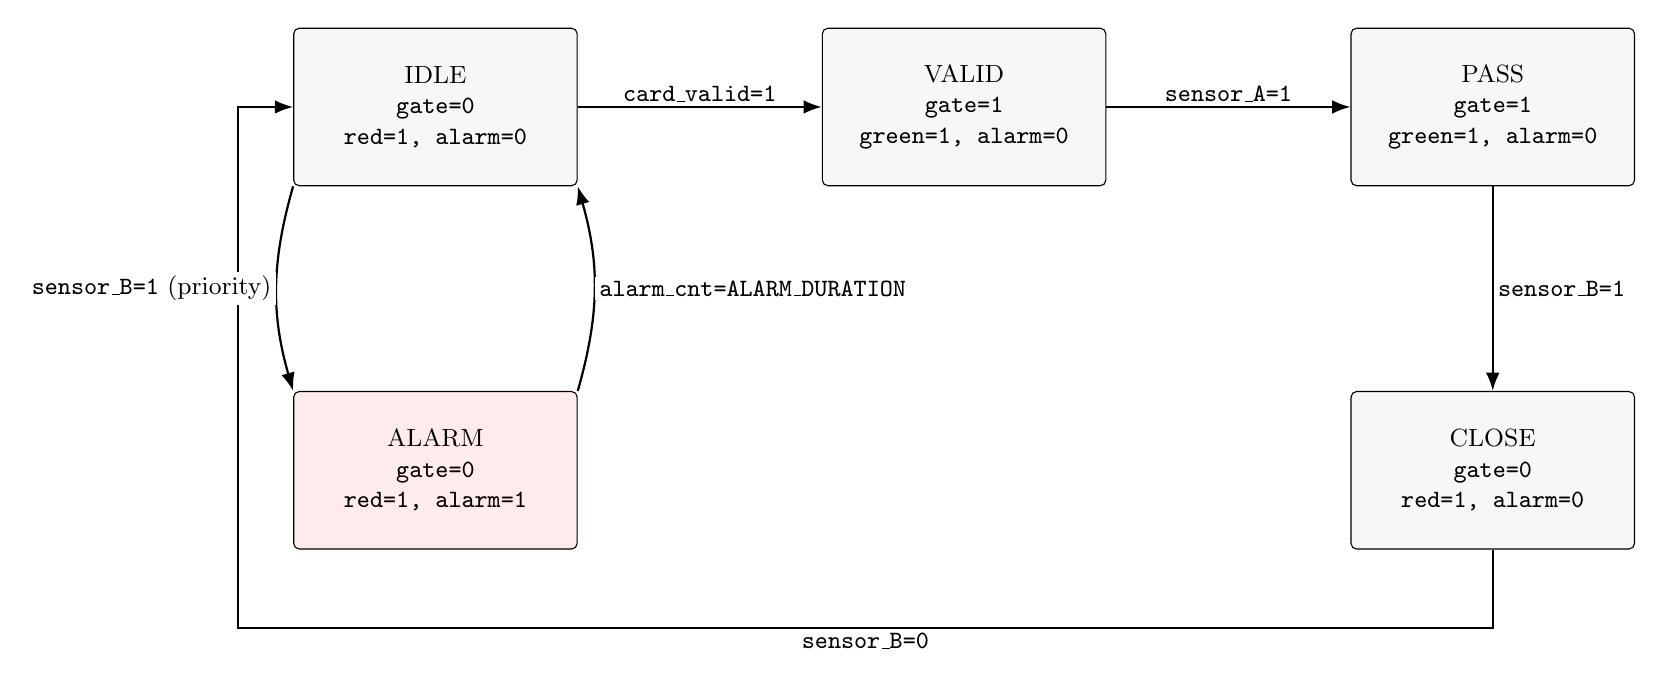
\begin{tikzpicture}
\node[fsmstate, minimum width=36mm, minimum height=20mm] (idle)
  {IDLE\\\texttt{gate=0}\\\texttt{red=1, alarm=0}};
\node[fsmstate, minimum width=36mm, minimum height=20mm, right=31mm of idle] (valid)
  {VALID\\\texttt{gate=1}\\\texttt{green=1, alarm=0}};
\node[fsmstate, minimum width=36mm, minimum height=20mm, right=31mm of valid] (pass)
  {PASS\\\texttt{gate=1}\\\texttt{green=1, alarm=0}};
\node[fsmstate, minimum width=36mm, minimum height=20mm, below=26mm of pass] (close)
  {CLOSE\\\texttt{gate=0}\\\texttt{red=1, alarm=0}};
\node[alarmstate, minimum width=36mm, minimum height=20mm, below=26mm of idle] (alarm)
  {ALARM\\\texttt{gate=0}\\\texttt{red=1, alarm=1}};
\coordinate[left=7mm of idle.west] (p3idlein);
\draw[fsmedge] (idle) -- node[fsmlabel, above] {\texttt{card\_valid=1}} (valid);
\draw[fsmedge] (valid) -- node[fsmlabel, above] {\texttt{sensor\_A=1}} (pass);
\draw[fsmedge] (pass) -- node[fsmlabel, right] {\texttt{sensor\_B=1}} (close);
\draw[fsmedge] (close.south) -- ++(0,-10mm) -| node[fsmlabel, pos=0.25, below] {\texttt{sensor\_B=0}} (p3idlein) -- (idle.west);
\draw[fsmedge] (idle.south west) to[bend right=16] node[fsmlabel, left] {\texttt{sensor\_B=1} (priority)} (alarm.north west);
\draw[fsmedge] (alarm.north east) to[bend right=16] node[fsmlabel, right] {\texttt{alarm\_cnt=ALARM\_DURATION}} (idle.south east);
\end{tikzpicture}%
}}

\newcommand{\PartFourFSM}{%
\resizebox{\textwidth}{!}{%
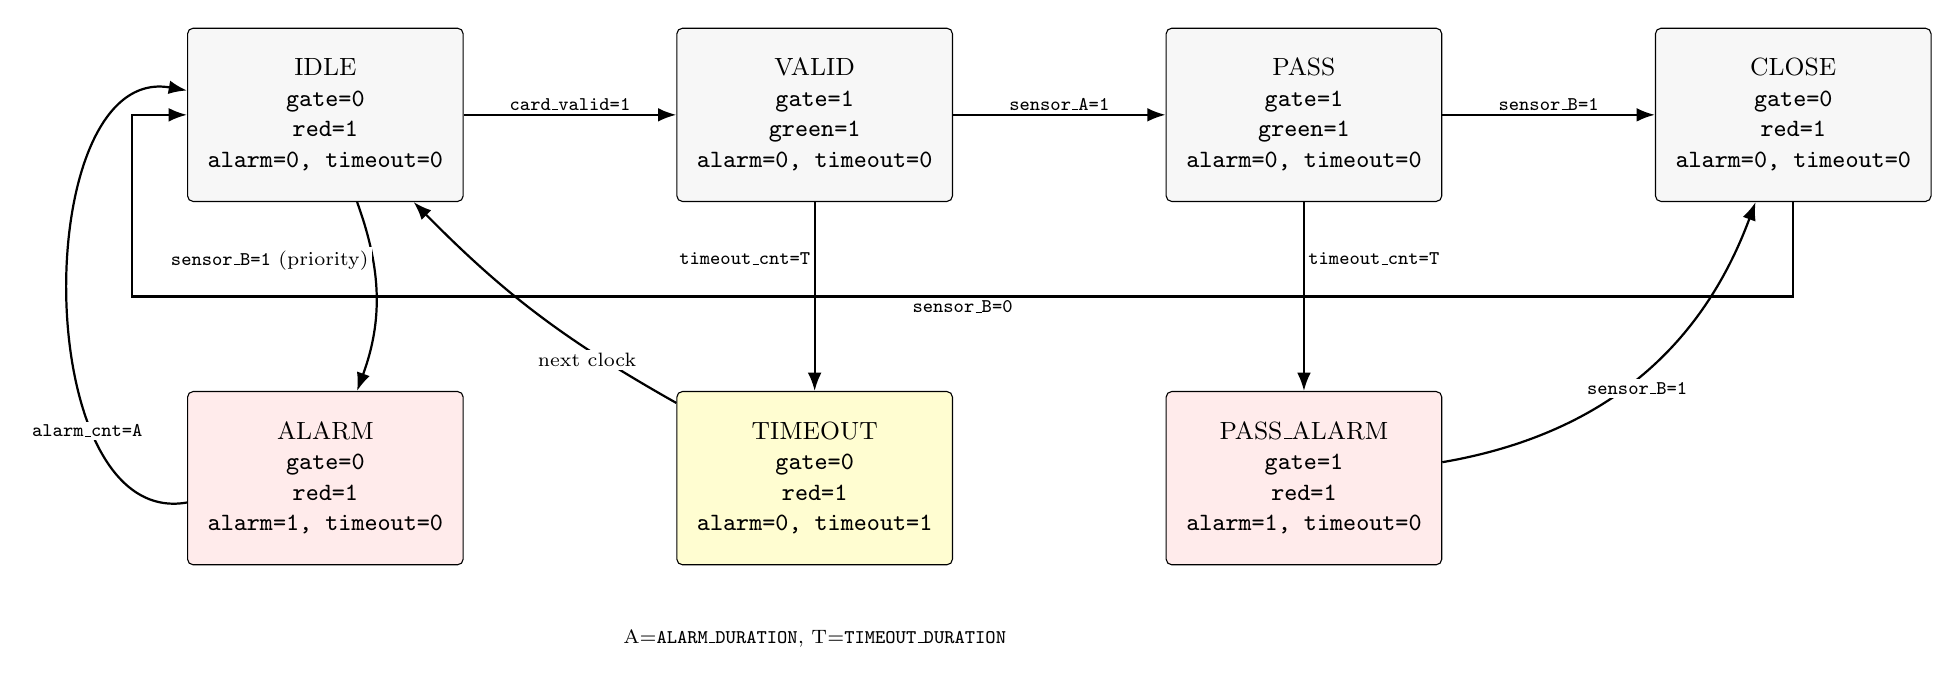
\begin{tikzpicture}
\tikzset{every node/.append style={font=\scriptsize}, fsmlabel/.style={font=\scriptsize, fill=white, inner sep=1.2pt}}
\node[fsmstate, minimum width=35mm, minimum height=22mm] (idle)
  {IDLE\\\texttt{gate=0}\\\texttt{red=1}\\\texttt{alarm=0, timeout=0}};
\node[fsmstate, minimum width=35mm, minimum height=22mm, right=27mm of idle] (valid)
  {VALID\\\texttt{gate=1}\\\texttt{green=1}\\\texttt{alarm=0, timeout=0}};
\node[fsmstate, minimum width=35mm, minimum height=22mm, right=27mm of valid] (pass)
  {PASS\\\texttt{gate=1}\\\texttt{green=1}\\\texttt{alarm=0, timeout=0}};
\node[fsmstate, minimum width=35mm, minimum height=22mm, right=27mm of pass] (close)
  {CLOSE\\\texttt{gate=0}\\\texttt{red=1}\\\texttt{alarm=0, timeout=0}};
\node[alarmstate, minimum width=35mm, minimum height=22mm, below=24mm of idle] (alarm)
  {ALARM\\\texttt{gate=0}\\\texttt{red=1}\\\texttt{alarm=1, timeout=0}};
\node[timeoutstate, minimum width=35mm, minimum height=22mm, below=24mm of valid] (timeout)
  {TIMEOUT\\\texttt{gate=0}\\\texttt{red=1}\\\texttt{alarm=0, timeout=1}};
\node[alarmstate, minimum width=35mm, minimum height=22mm, below=24mm of pass] (passalarm)
  {PASS\_ALARM\\\texttt{gate=1}\\\texttt{red=1}\\\texttt{alarm=1, timeout=0}};
\coordinate[left=7mm of idle.west] (p4idlein);
\draw[fsmedge] (idle) -- node[fsmlabel, above] {\texttt{card\_valid=1}} (valid);
\draw[fsmedge] (valid) -- node[fsmlabel, above] {\texttt{sensor\_A=1}} (pass);
\draw[fsmedge] (pass) -- node[fsmlabel, above] {\texttt{sensor\_B=1}} (close);
\draw[fsmedge] (close.south) -- ++(0,-12mm) -| node[fsmlabel, pos=0.25, below] {\texttt{sensor\_B=0}} (p4idlein) -- (idle.west);
\draw[fsmedge] (idle) to[bend left=20] node[fsmlabel, left ,pos=0.3] {\texttt{sensor\_B=1} (priority)} (alarm);
\draw[fsmedge] (alarm) to[bend left=100] node[fsmlabel, below, pos = 0.3] {\texttt{alarm\_cnt=A}} (idle);
\draw[fsmedge] (valid) -- node[fsmlabel, left, pos=0.3] {\texttt{timeout\_cnt=T}} (timeout);
\draw[fsmedge] (timeout) to[bend left=8] node[fsmlabel, below, pos=0.3] {next clock} (idle);
\draw[fsmedge] (pass) -- node[fsmlabel, right, pos=0.3] {\texttt{timeout\_cnt=T}} (passalarm);
\draw[fsmedge] (passalarm) to[bend right=30] node[fsmlabel, below] {\texttt{sensor\_B=1}} (close);
\node[font=\scriptsize, below=7mm of timeout] {A=\texttt{ALARM\_DURATION}, T=\texttt{TIMEOUT\_DURATION}};
\end{tikzpicture}%
}}

% ── title ──
\title{\textbf{Subway Turnstile Controller Report}}
\author{古明地雷\quad (114514)}
\date{\today}

\begin{document}

\maketitle
\thispagestyle{empty}

\vspace{-1.5em}
\begin{center}
\rule{0.9\textwidth}{0.5pt}\\[0.3em]
{\small \textbf{ShanghaiTech University · EE115B Digital Circuit Design}}
\end{center}

\section*{Overview}

This report documents the Moore FSM design, state diagrams, simulation
waveforms, and verification results for all four parts of the subway
turnstile controller project. All Verilog modules were simulated with
Icarus Verilog 11.0. State diagrams are drawn directly in TikZ,
waveforms were generated from VCD dumps, and the report is typeset
with \LaTeX{}.

\medskip
\noindent\textbf{Design conventions}:
\begin{itemize}[nosep]
  \item Asynchronous active-low reset (\texttt{rst\_n}) in every module.
  \item \texttt{sensor\_B} $>$ \texttt{card\_valid} priority in IDLE
        (Part~3/4).
  \item Parameterized delay values: \texttt{ALARM\_DURATION} and
        \texttt{TIMEOUT\_DURATION}.
\end{itemize}

\newpage

% ━━━━━━━━━━━━━━━━━━━━━━━━━━━━━━━━━━━━━━━━━━━━━━━━━━
\section{Part 1: Two-State Turnstile}

A two-state Moore FSM is used. \texttt{LOCKED} keeps the gate closed
with the red LED on. A valid card moves the controller to
\texttt{UNLOCKED}, which opens the gate and enables passage.
\texttt{sensor\_B} closes the gate after the passenger exits.

\subsection*{Signal Interface}
\begin{tabular}{llll}
\toprule
\textbf{Signal} & \textbf{Dir} & \textbf{W} & \textbf{Description} \\
\midrule
\texttt{clk}       & Input  & 1 & System clock \\
\texttt{rst\_n}    & Input  & 1 & Asynch.\ active-low reset \\
\texttt{card\_valid} & Input  & 1 & Card tap pulse \\
\texttt{sensor\_B} & Input  & 1 & Rear IR sensor \\
\texttt{gate\_open} & Output & 1 & Gate control (1=open) \\
\texttt{led\_green} & Output & 1 & Green passage LED \\
\texttt{led\_red}   & Output & 1 & Red stop LED \\
\bottomrule
\end{tabular}

\subsection*{State Encoding}
\begin{tabular}{lll}
\toprule
\textbf{State} & \textbf{Code} & \textbf{Outputs} \\
\midrule
LOCKED   & 0 & gate=0, green=0, red=1 \\
UNLOCKED & 1 & gate=1, green=1, red=0 \\
\bottomrule
\end{tabular}

\subsection*{State Diagram}
\begin{figure}[H]
\centering
\PartOneFSM
\caption{Part~1 FSM (2 states)}
\end{figure}

\subsection*{Simulation Waveform}
\begin{figure}[H]
\centering
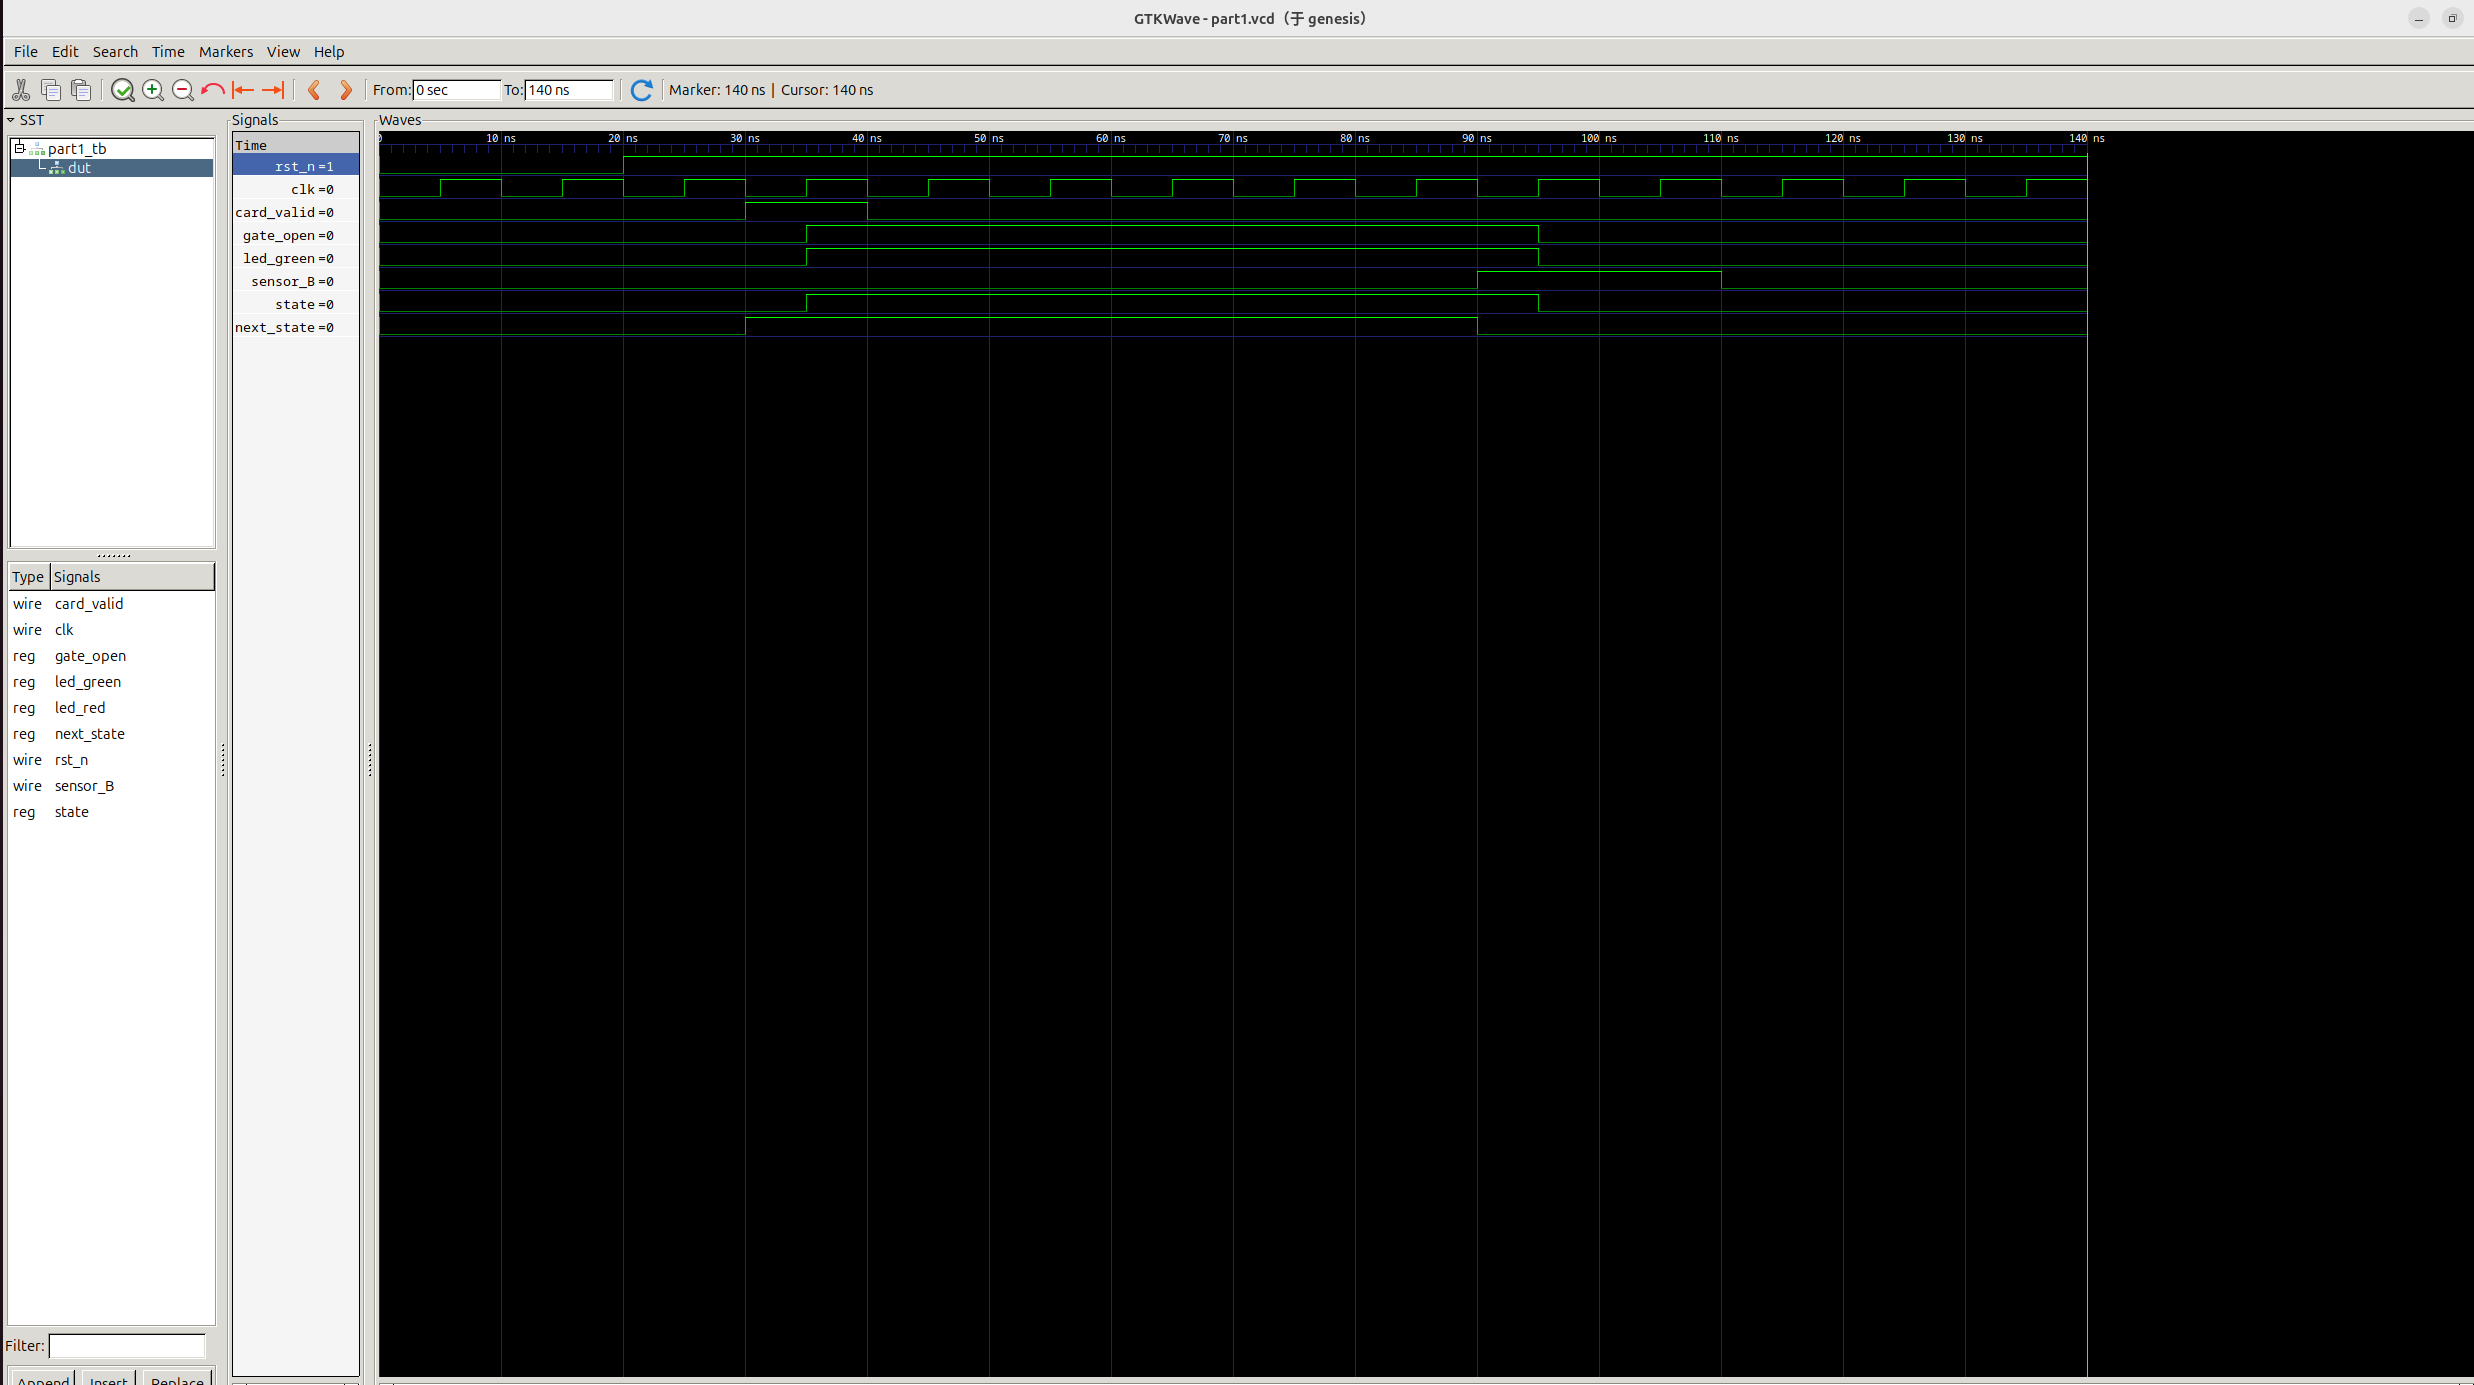
\includegraphics[width=\textwidth]{part1.png}
\caption{card\_valid opens the gate; sensor\_B closes it}
\end{figure}

\subsection*{Verification}
{\color{passgreen}\textbf{Compile: PASS} $\;|\;$
 \textbf{Simulate: PASS} $\;|\;$
 \textbf{Result: PASS}}

card\_valid opens the gate (green LED on); sensor\_B closes the gate
(red LED on). Reset holds the state at LOCKED.

\newpage

% ━━━━━━━━━━━━━━━━━━━━━━━━━━━━━━━━━━━━━━━━━━━━━━━━━━
\section{Part 2: Basic Access Control}

The controller is extended to a four-state Moore FSM. \texttt{IDLE}
waits for a card, \texttt{VALID} waits for lane entry at sensor\_A,
\texttt{PASS} waits for exit at sensor\_B, and \texttt{CLOSE} holds
the gate shut until sensor\_B is released.

\subsection*{Signal Interface}
\begin{tabular}{llll}
\toprule
\textbf{Signal} & \textbf{Dir} & \textbf{W} & \textbf{Description} \\
\midrule
\texttt{clk}       & Input  & 1 & System clock \\
\texttt{rst\_n}    & Input  & 1 & Asynch.\ active-low reset \\
\texttt{card\_valid} & Input  & 1 & Card tap (only valid in IDLE) \\
\texttt{sensor\_A} & Input  & 1 & Front IR sensor \\
\texttt{sensor\_B} & Input  & 1 & Rear IR sensor \\
\texttt{gate\_open} & Output & 1 & Gate control \\
\texttt{led\_green} & Output & 1 & Green passage LED \\
\texttt{led\_red}   & Output & 1 & Red stop LED \\
\bottomrule
\end{tabular}

\subsection*{State Encoding}
\begin{tabular}{lll}
\toprule
\textbf{State} & \textbf{Code} & \textbf{Outputs} \\
\midrule
IDLE  & 00 & gate=0, red=1 \\
VALID & 01 & gate=1, green=1 \\
PASS  & 10 & gate=1, green=1 \\
CLOSE & 11 & gate=0, red=1 \\
\bottomrule
\end{tabular}

\subsection*{State Diagram}
\begin{figure}[H]
\centering
\PartTwoFSM
\caption{Part~2 FSM (4 states)}
\end{figure}

\subsection*{Simulation Waveform}
\begin{figure}[H]
\centering
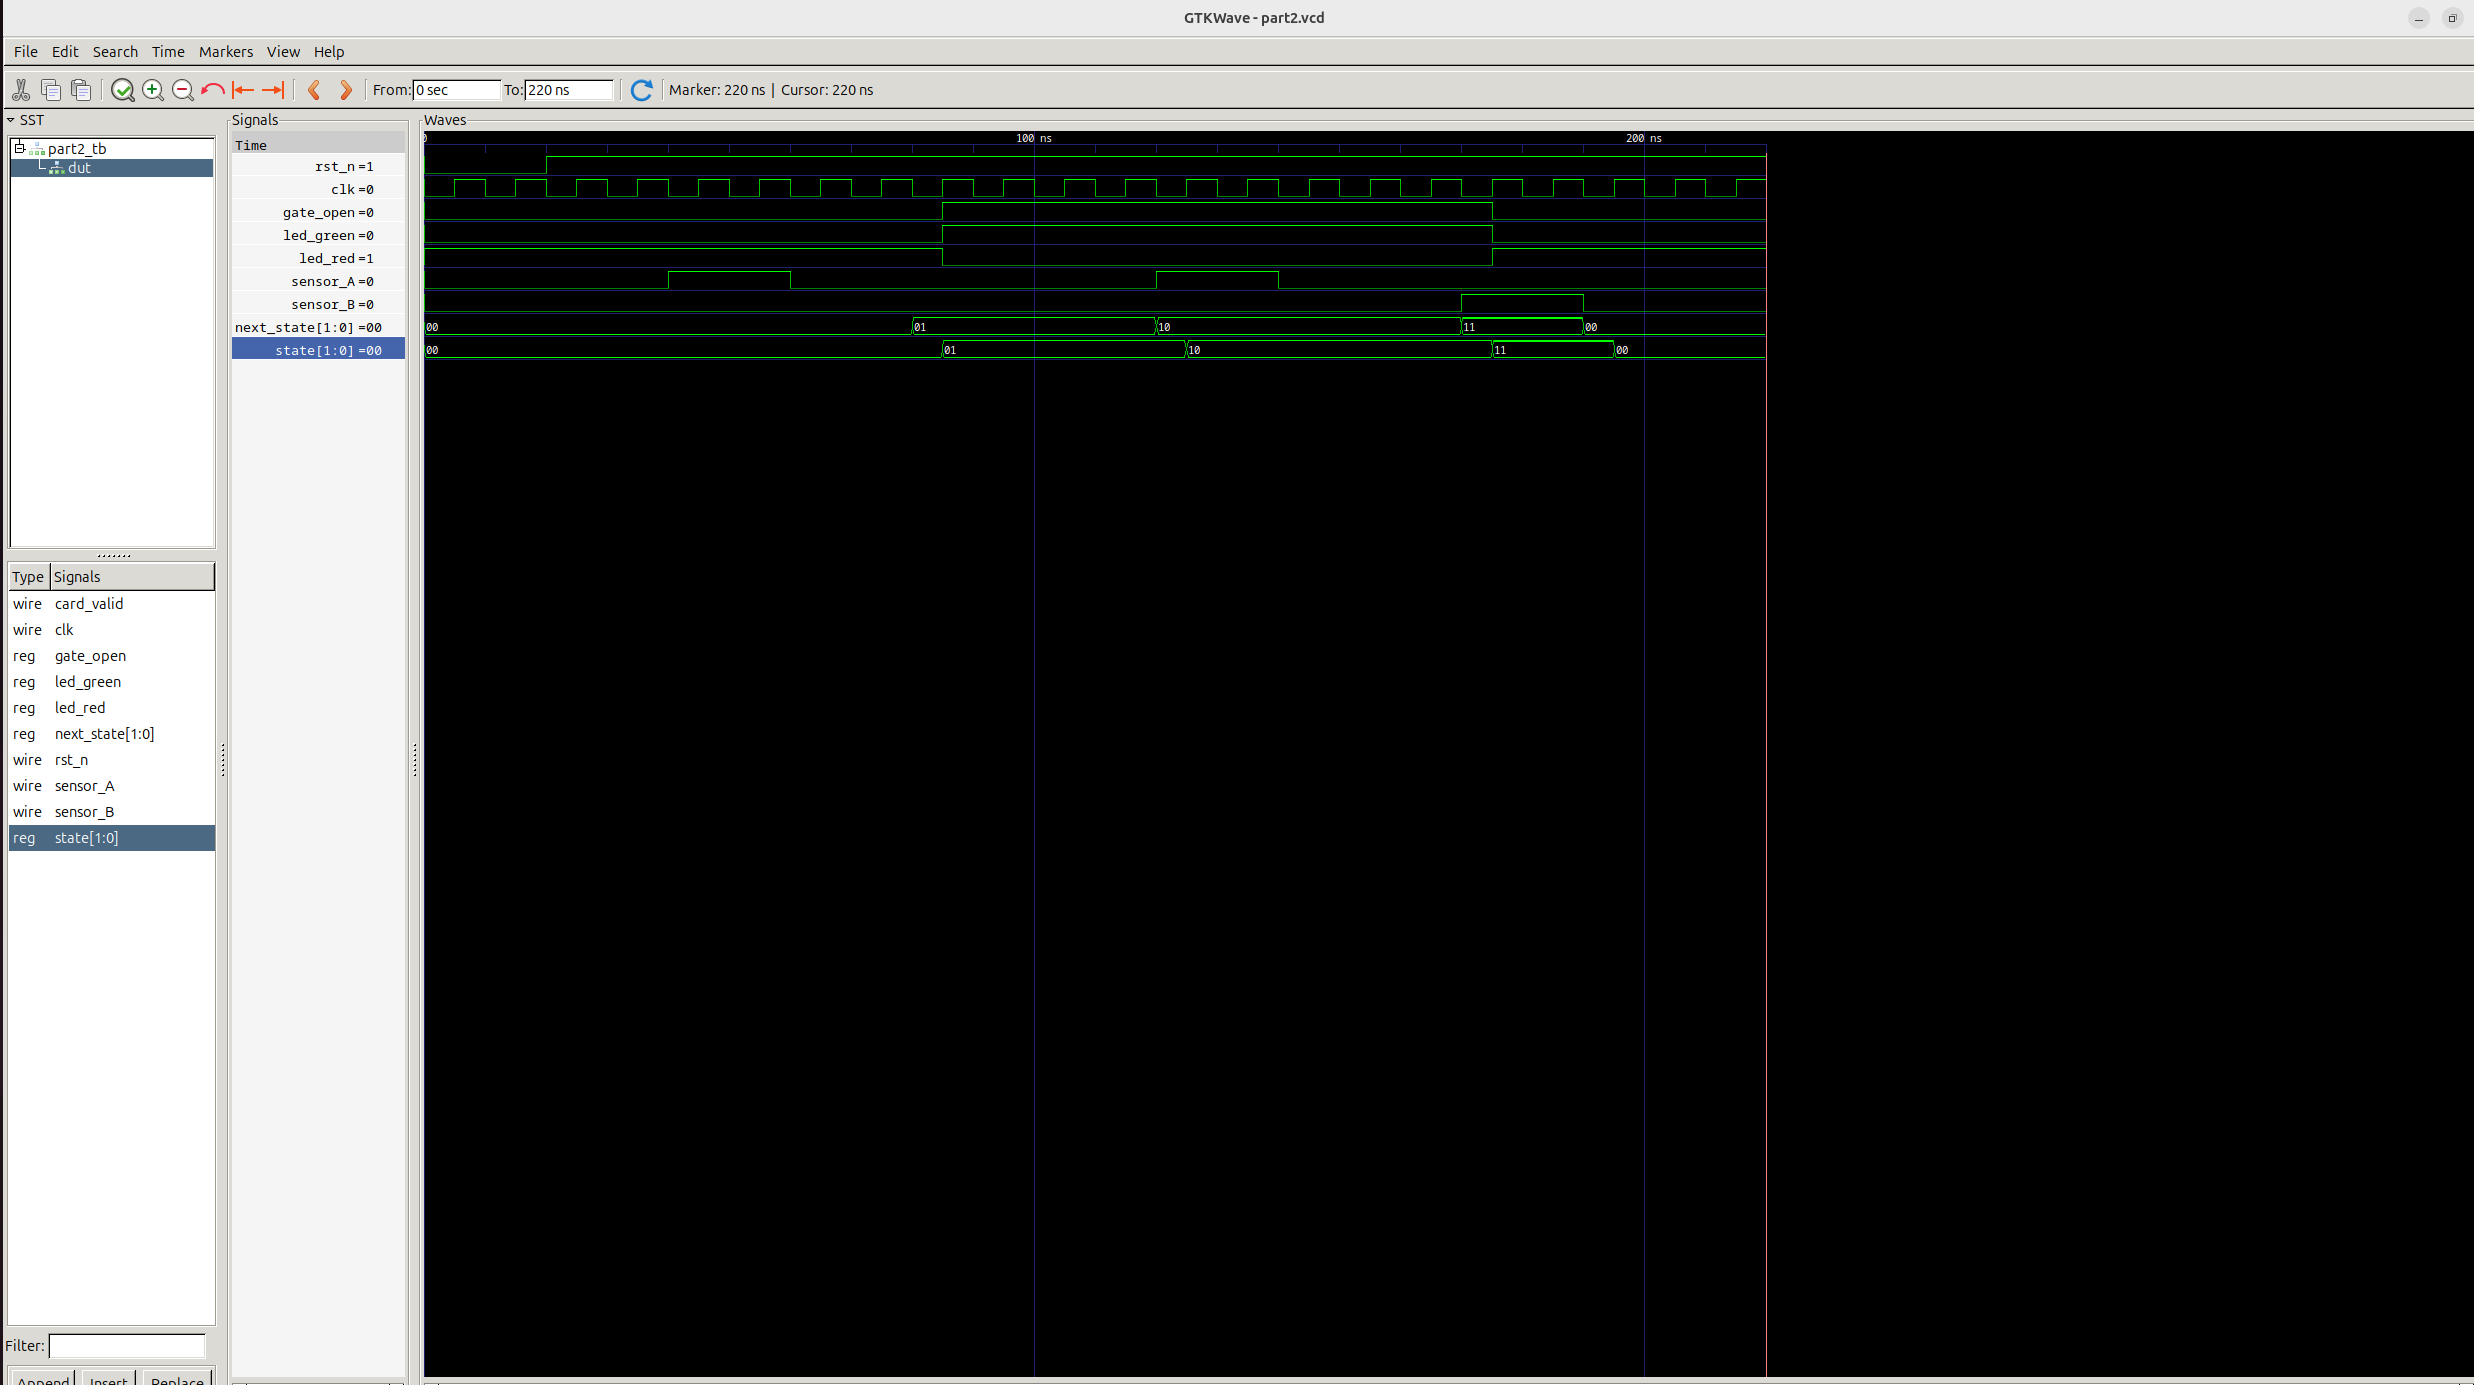
\includegraphics[width=\textwidth]{part2.png}
\caption{sensor\_A ignored in IDLE; normal card-to-exit passage}
\end{figure}

\subsection*{Verification}
{\color{passgreen}\textbf{Compile: PASS} $\;|\;$
 \textbf{Simulate: PASS} $\;|\;$
 \textbf{Result: PASS}}

sensor\_A is correctly ignored in IDLE (gate stays closed). The full
forward chain (card → VALID → sensor\_A → PASS → sensor\_B → CLOSE →
sensor\_B=0 → IDLE) is confirmed. Student-written testbench
(\texttt{part2\_tb.v}) covers both edge cases.

\newpage

% ━━━━━━━━━━━━━━━━━━━━━━━━━━━━━━━━━━━━━━━━━━━━━━━━━━
\section{Part 3: Reverse Intrusion Detection}

Part~3 adds an \texttt{ALARM} state and an alarm counter. In
\texttt{IDLE}, \texttt{sensor\_B} has higher priority than
\texttt{card\_valid}, so reverse intrusion is detected before any card
action. The alarm stays high for \texttt{ALARM\_DURATION} clock
cycles, while the gate remains closed and the red LED remains on.

\subsection*{Signal Interface}
\begin{tabular}{llll}
\toprule
\textbf{Signal} & \textbf{Dir} & \textbf{W} & \textbf{Description} \\
\midrule
\texttt{clk}       & Input  & 1 & System clock \\
\texttt{rst\_n}    & Input  & 1 & Asynch.\ active-low reset \\
\texttt{card\_valid} & Input  & 1 & Card tap (only valid in IDLE) \\
\texttt{sensor\_A} & Input  & 1 & Front IR sensor \\
\texttt{sensor\_B} & Input  & 1 & Rear IR sensor (priority in IDLE) \\
\texttt{gate\_open} & Output & 1 & Gate control \\
\texttt{led\_green} & Output & 1 & Green passage LED \\
\texttt{led\_red}   & Output & 1 & Red stop LED \\
\texttt{alarm}     & Output & 1 & Reverse intrusion alarm \\
\bottomrule
\end{tabular}

\subsection*{Parameters}
\begin{tabular}{lll}
\toprule
\textbf{Name} & \textbf{Value} & \textbf{Notes} \\
\midrule
\texttt{ALARM\_DURATION} & 10 & Alarm clock cycles \\
\bottomrule
\end{tabular}

\subsection*{State Encoding}
\begin{tabular}{lll}
\toprule
\textbf{State} & \textbf{Code} & \textbf{Outputs} \\
\midrule
IDLE  & 000 & gate=0, alarm=0 \\
VALID & 001 & gate=1, alarm=0 \\
PASS  & 010 & gate=1, alarm=0 \\
CLOSE & 011 & gate=0, alarm=0 \\
ALARM & 100 & gate=0, alarm=1 \\
\bottomrule
\end{tabular}

\subsection*{State Diagram}
\begin{figure}[H]
\centering
\PartThreeFSM
\caption{Part~3 FSM (5 states, ALARM added)}
\end{figure}

\subsection*{Simulation Waveform}
\begin{figure}[H]
\centering
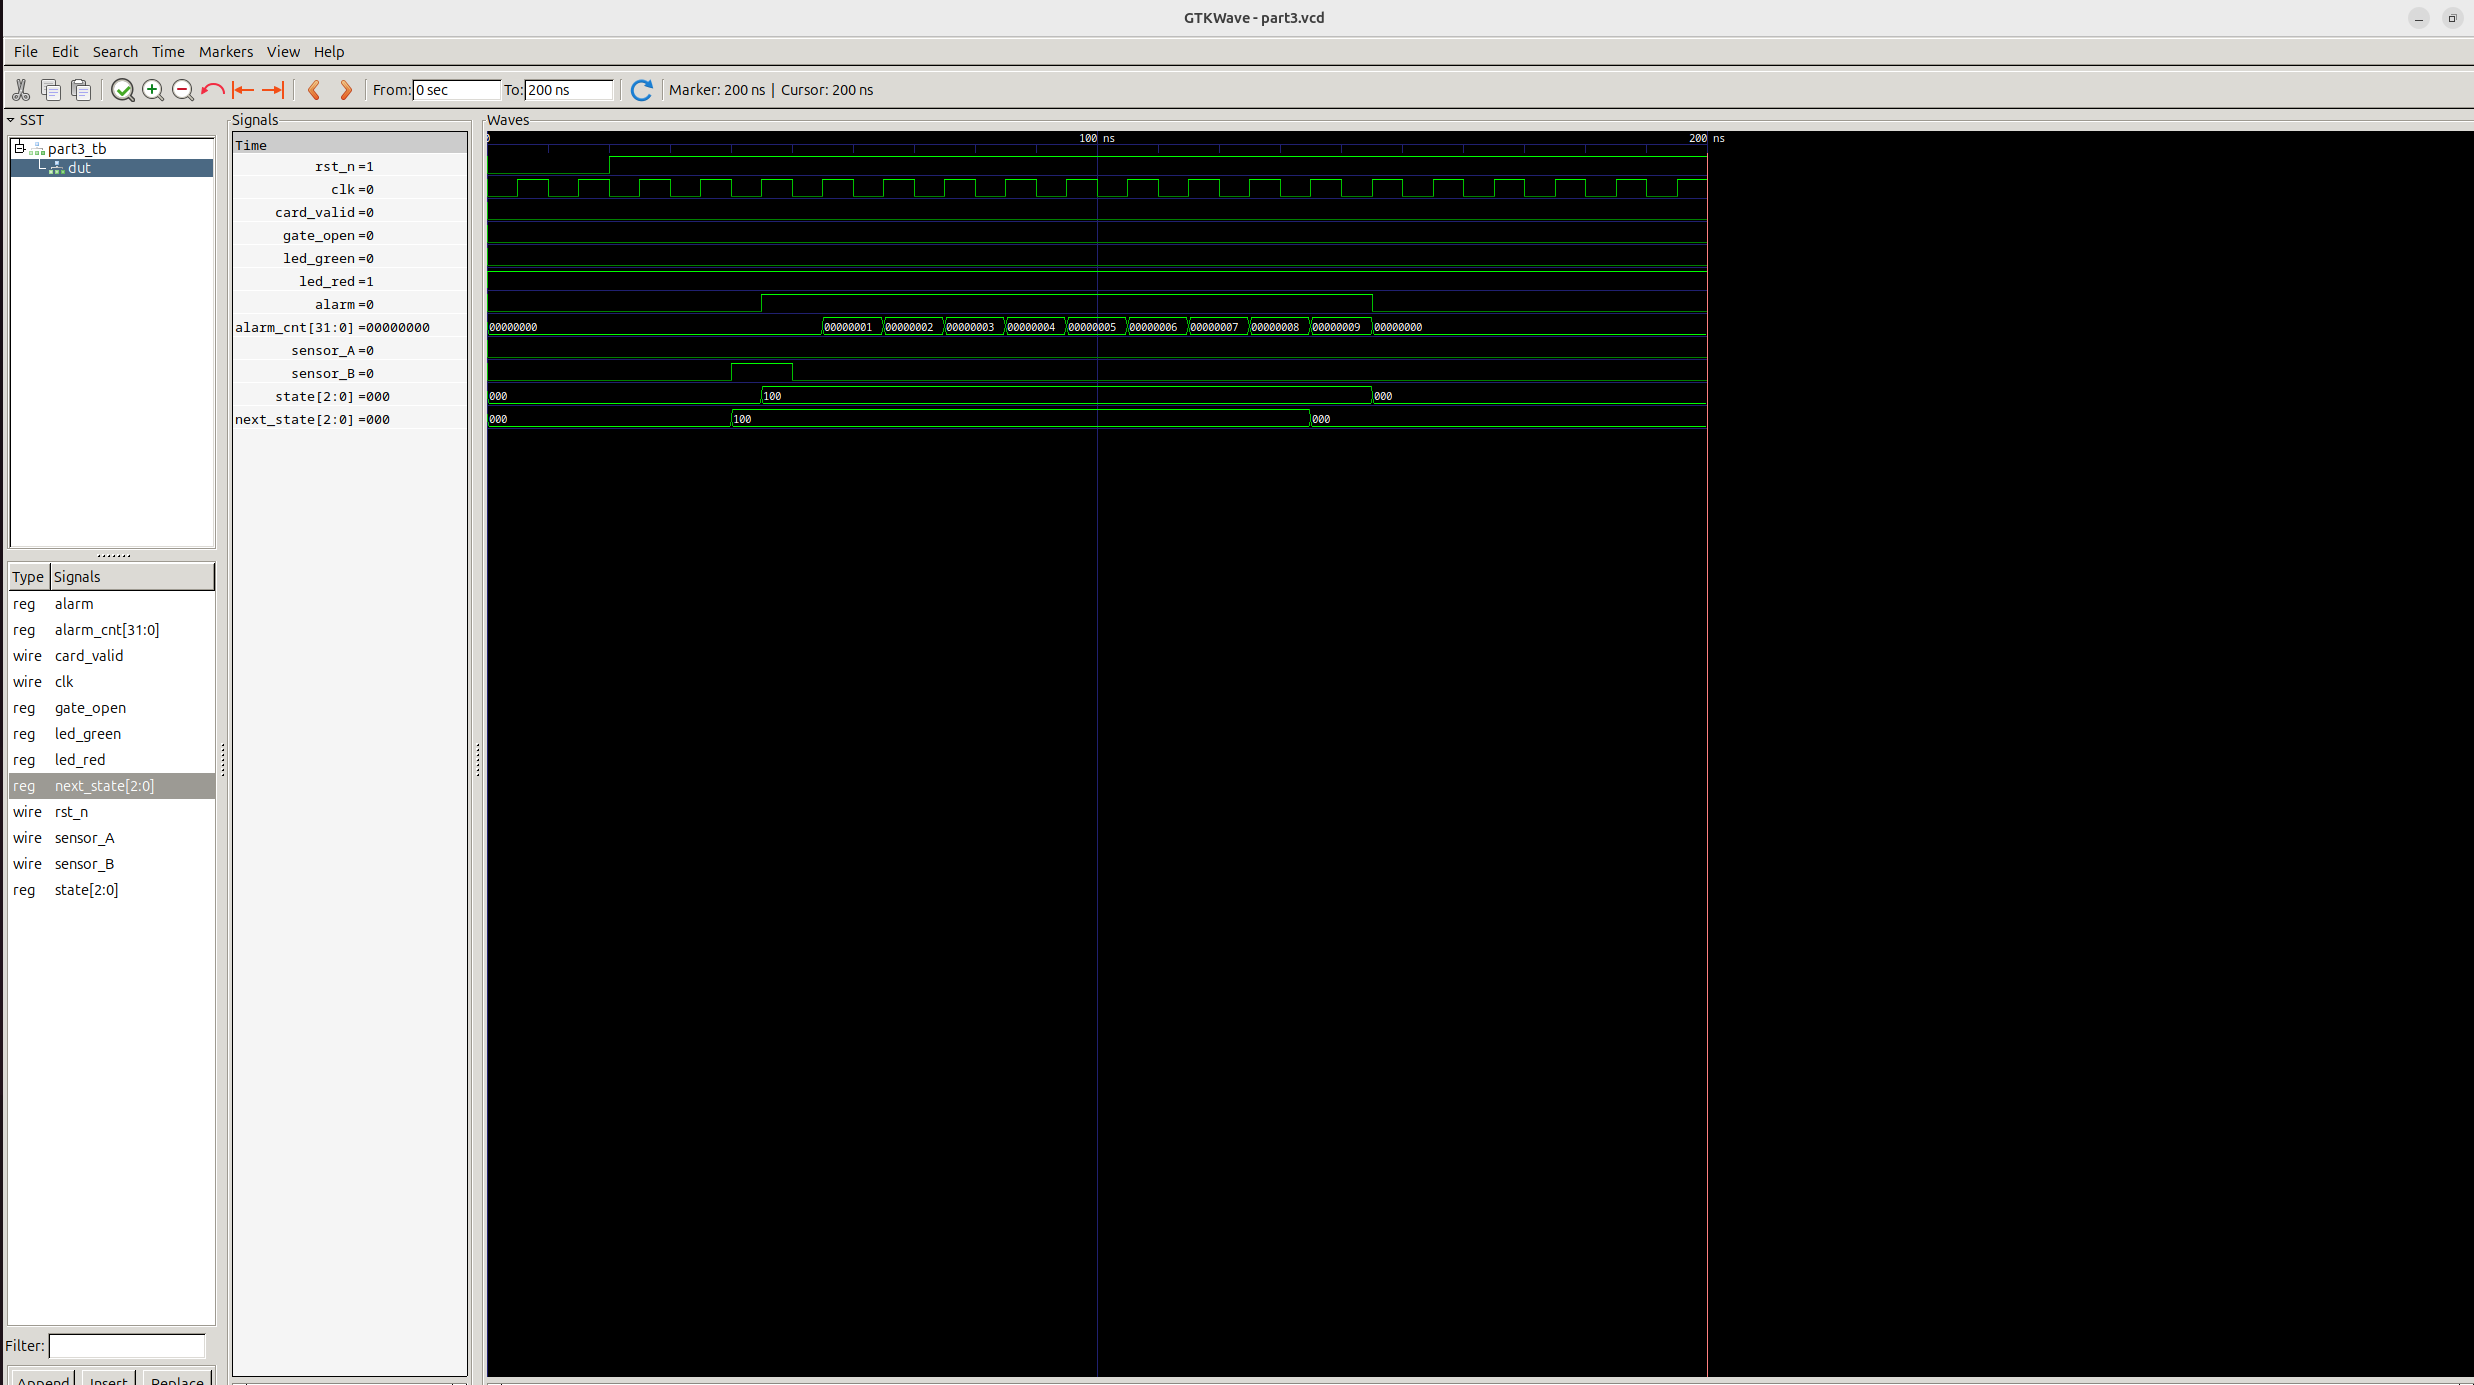
\includegraphics[width=\textwidth]{part3.png}
\caption{sensor\_B in IDLE triggers ALARM (10 cycles, priority over card\_valid)}
\end{figure}

\subsection*{Verification}
{\color{passgreen}\textbf{Compile: PASS} $\;|\;$
 \textbf{Simulate: PASS} $\;|\;$
 \textbf{Result: PASS}}

sensor\_B=1 in IDLE triggers the ALARM state (priority over
card\_valid). Alarm duration: 10 clock cycles
(\texttt{ALARM\_DURATION}=10, verified via VCD). Gate stays closed and
red LED stays on throughout the entire ALARM period.

\newpage

% ━━━━━━━━━━━━━━━━━━━━━━━━━━━━━━━━━━━━━━━━━━━━━━━━━━
\section{Part 4: Timeout Auto-Close}

Part~4 retains the reverse-intrusion alarm and introduces two more
behaviors. In \texttt{VALID}, a timeout counter auto-closes the gate
and asserts \texttt{timeout} when no passenger enters before
\texttt{TIMEOUT\_DURATION}. In \texttt{PASS}, the same timeout
concept raises \texttt{PASS\_ALARM} if a passenger stays in the
lane too long. \texttt{PASS\_ALARM} keeps the gate open, drives alarm
high, and waits for \texttt{sensor\_B} before finishing through
\texttt{CLOSE}.

\subsection*{Signal Interface}
\begin{tabular}{llll}
\toprule
\textbf{Signal} & \textbf{Dir} & \textbf{W} & \textbf{Description} \\
\midrule
\texttt{clk}       & Input  & 1 & System clock \\
\texttt{rst\_n}    & Input  & 1 & Asynch.\ active-low reset \\
\texttt{card\_valid} & Input  & 1 & Card tap pulse \\
\texttt{sensor\_A} & Input  & 1 & Front IR sensor \\
\texttt{sensor\_B} & Input  & 1 & Rear IR sensor \\
\texttt{gate\_open} & Output & 1 & Gate control \\
\texttt{led\_green} & Output & 1 & Green passage LED \\
\texttt{led\_red}   & Output & 1 & Red stop LED \\
\texttt{alarm}     & Output & 1 & Reverse / stuck alarm \\
\texttt{timeout}   & Output & 1 & Timeout indicator \\
\bottomrule
\end{tabular}

\subsection*{Parameters}
\begin{tabular}{lll}
\toprule
\textbf{Name} & \textbf{Value} & \textbf{Notes} \\
\midrule
\texttt{ALARM\_DURATION}  & 10 & Alarm cycles \\
\texttt{TIMEOUT\_DURATION} & 10 & Timeout cycles \\
\bottomrule
\end{tabular}

\subsection*{State Encoding}
\begin{tabular}{lll}
\toprule
\textbf{State} & \textbf{Code} & \textbf{Outputs} \\
\midrule
IDLE       & 000 & gate=0, alarm=0, timeout=0 \\
VALID      & 001 & gate=1, alarm=0, timeout=0 \\
PASS       & 010 & gate=1, alarm=0, timeout=0 \\
CLOSE      & 011 & gate=0, alarm=0, timeout=0 \\
ALARM      & 100 & gate=0, alarm=1, timeout=0 \\
TIMEOUT    & 101 & gate=0, alarm=0, timeout=1 \\
PASS\_ALARM & 110 & gate=1, alarm=1, timeout=0 \\
\bottomrule
\end{tabular}

\subsection*{State Diagram}
\begin{figure}[H]
\centering
\PartFourFSM
\caption{Part~4 FSM (7 states, TIMEOUT and PASS\_ALARM added)}
\end{figure}

\subsection*{Simulation Waveform --- Timeout Case}
\begin{figure}[H]
\centering
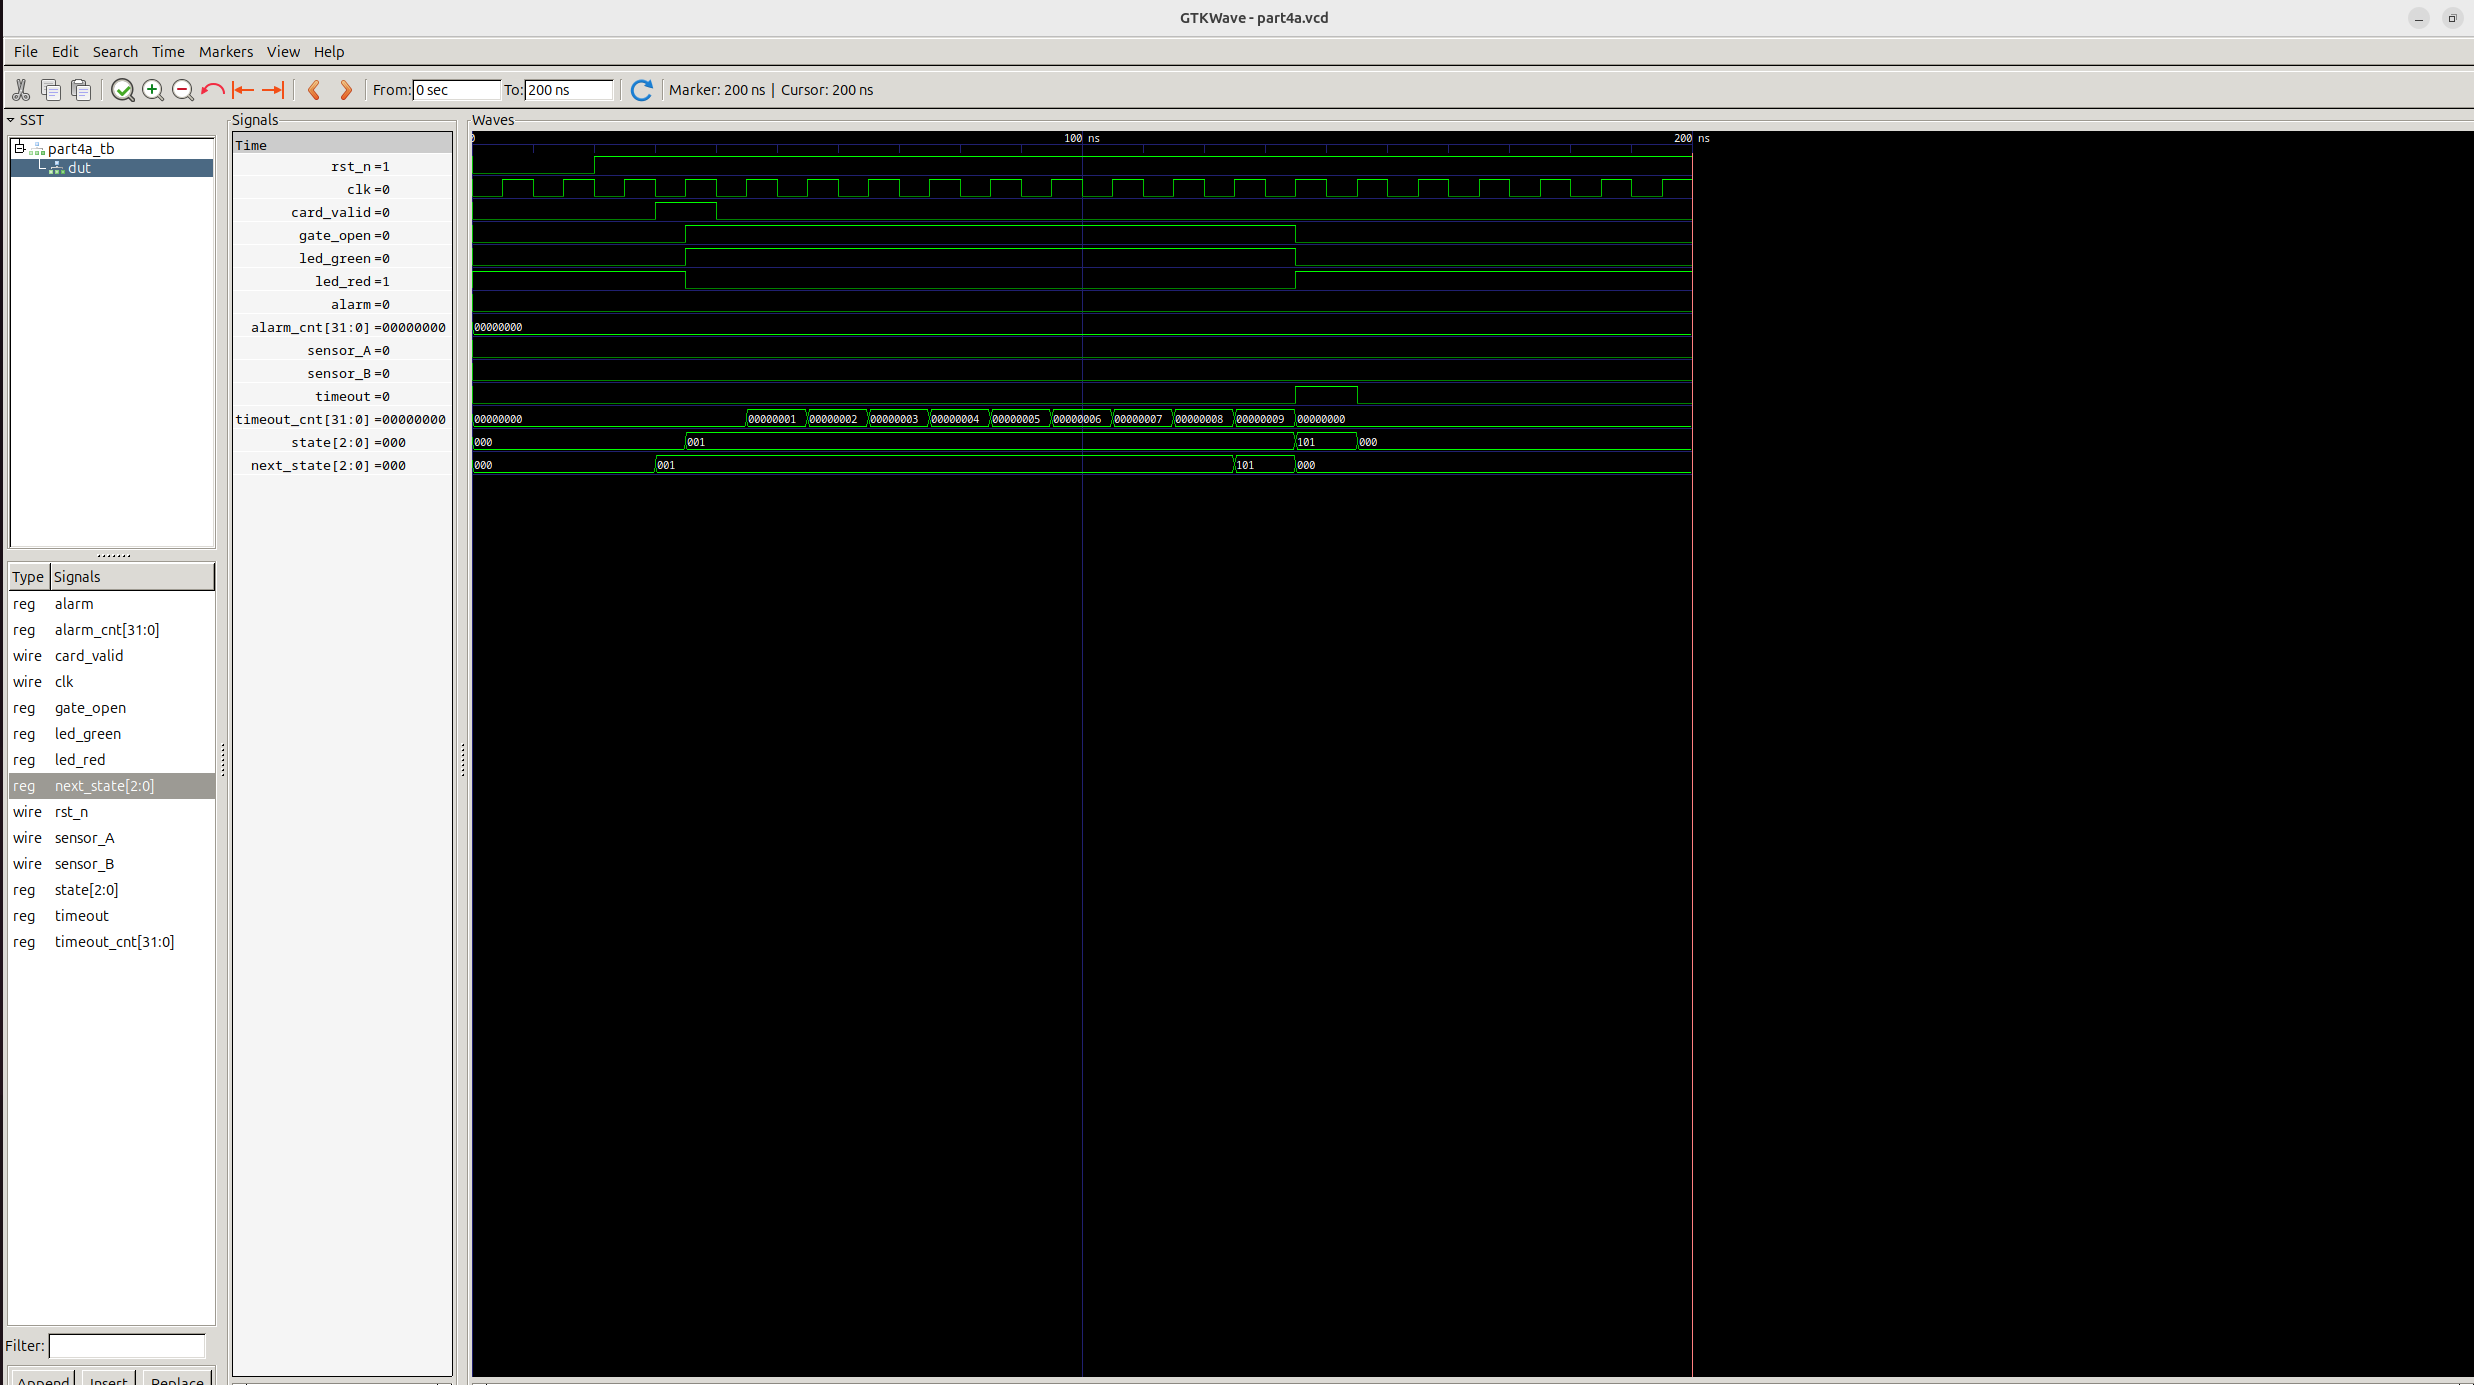
\includegraphics[width=\textwidth]{part4a.png}
\caption{card\_valid→VALID, no sensor\_A for 10 cycles→TIMEOUT (timeout=1)}
\end{figure}

\subsection*{Simulation Waveform --- Normal Passage Case}
\begin{figure}[H]
\centering
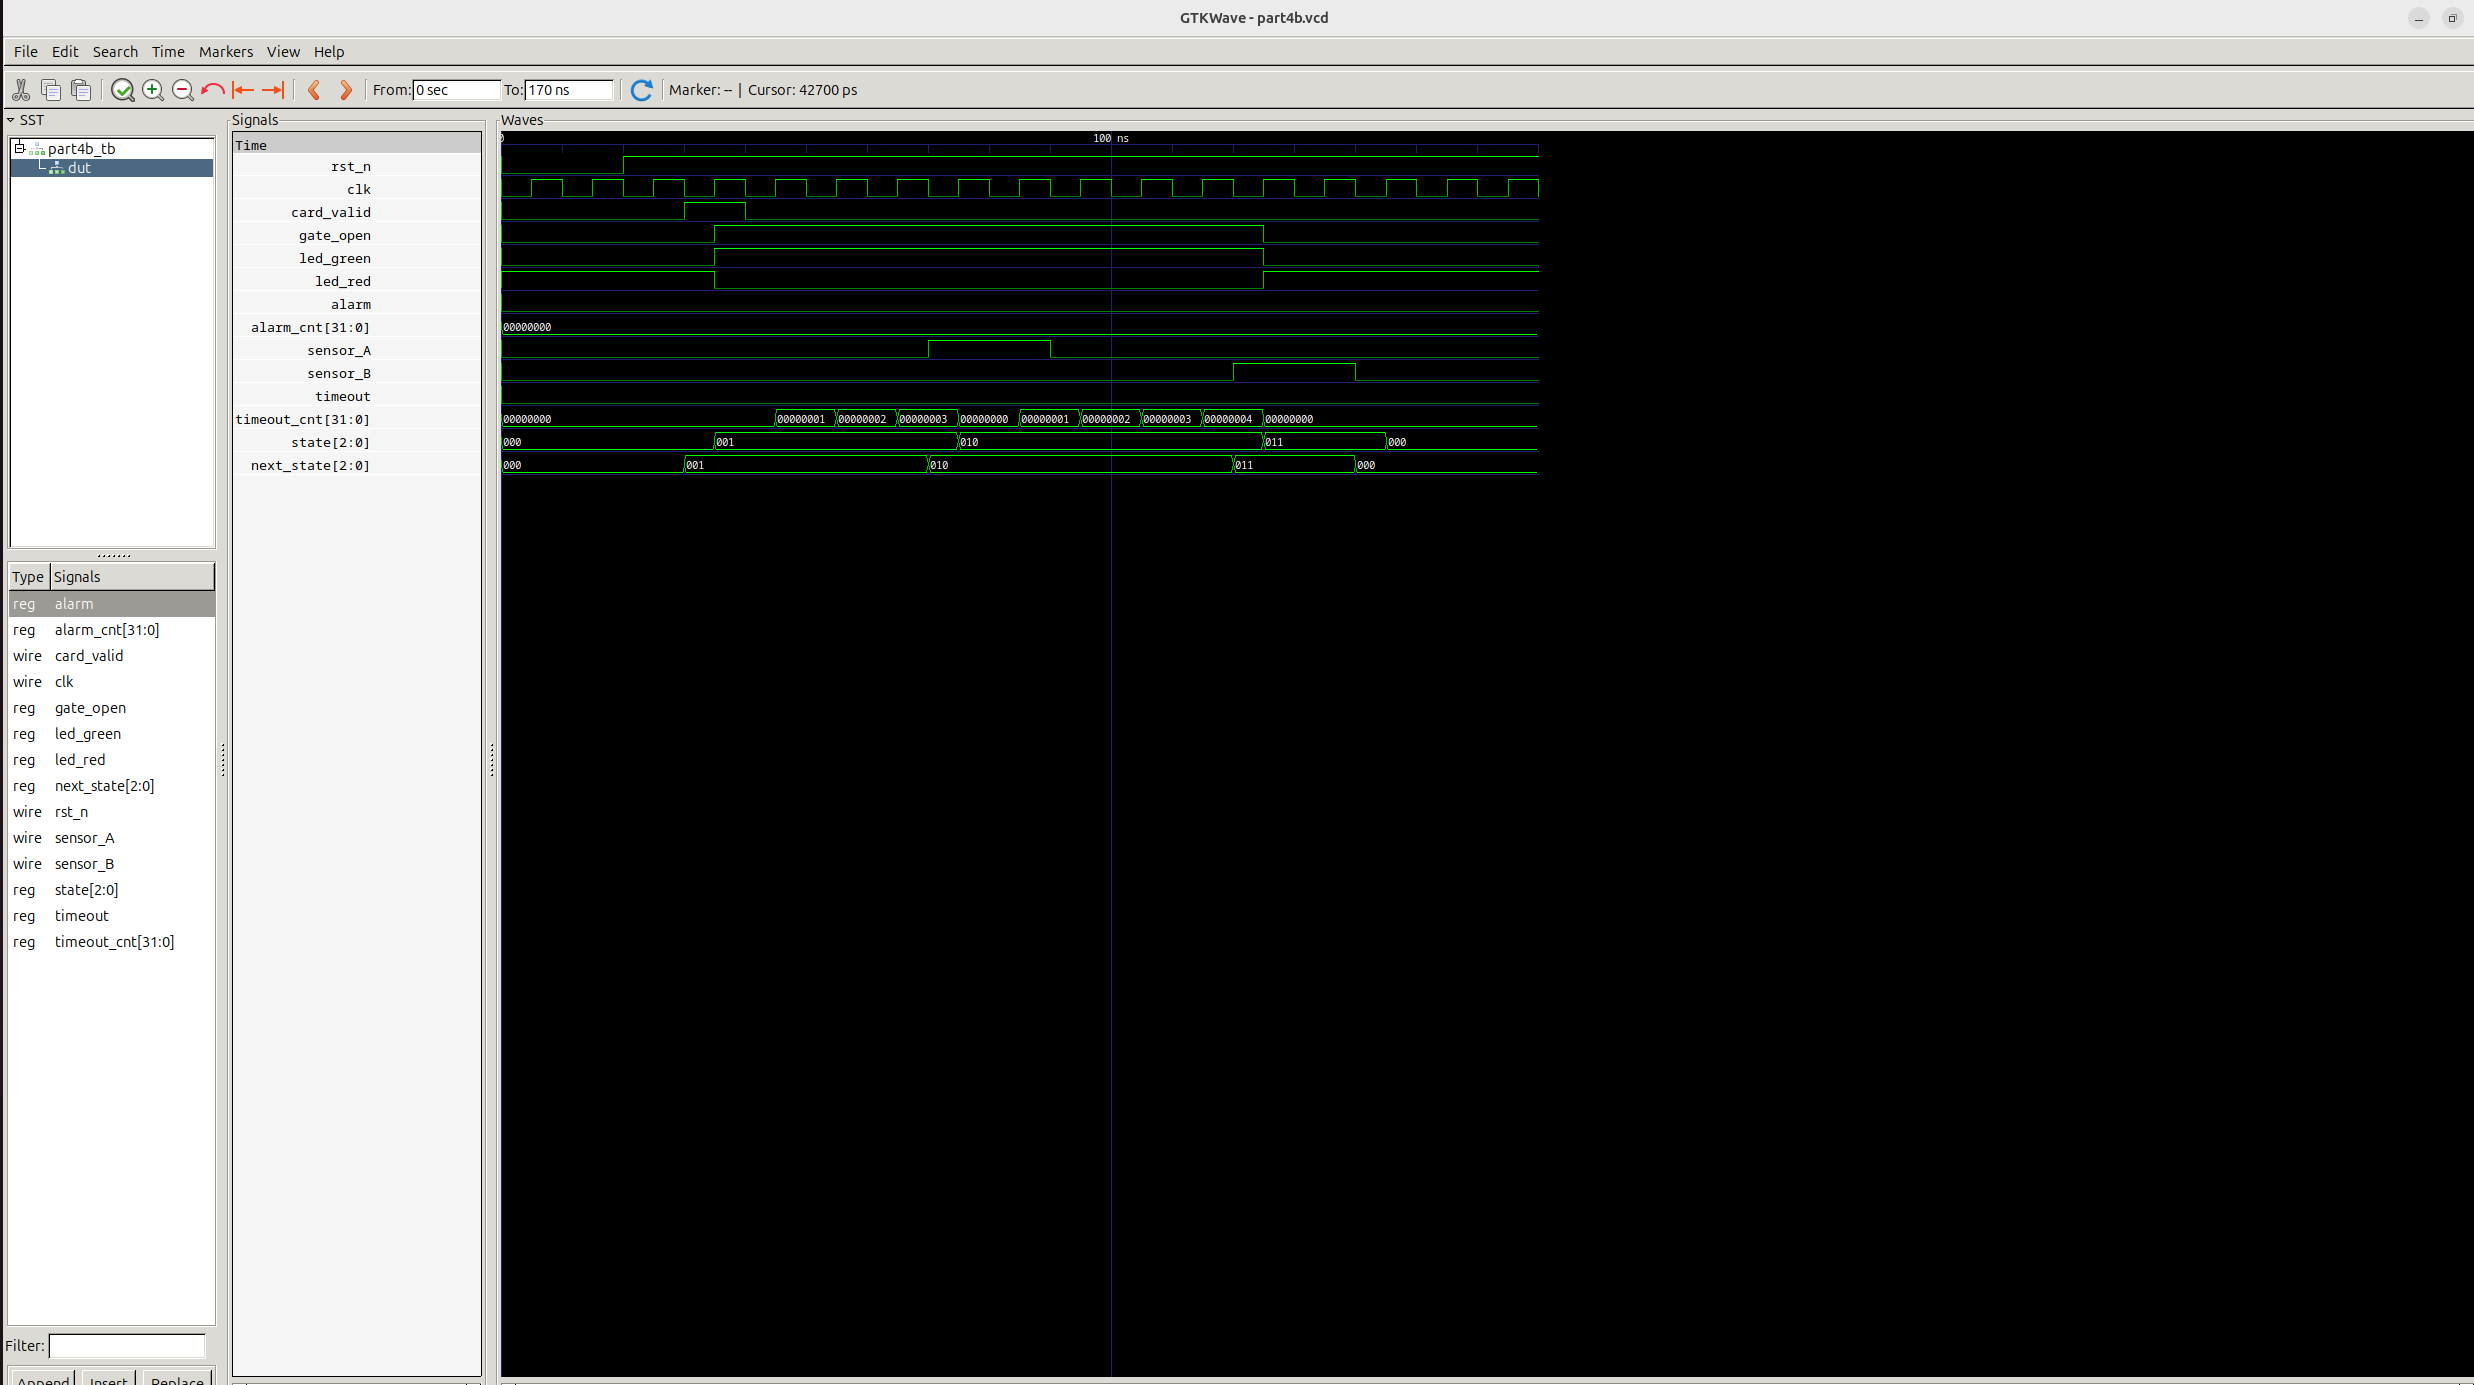
\includegraphics[width=\textwidth]{part4b.png}
\caption{card→sensor\_A→sensor\_B, no alarm, no timeout}
\end{figure}

\subsection*{Verification}
{\color{passgreen}\textbf{Compile: PASS} $\;|\;$
 \textbf{Simulate: PASS} $\;|\;$
 \textbf{Result: PASS}}

Timeout case (4a): after a valid card, no sensor\_A activity for 10 cycles
enters the timeout state with timeout=1, then returns to IDLE on the next clock.
Normal case (4b): card → sensor\_A → sensor\_B completes passage with no
alarm and no timeout. Both student-written testbenches verify correct behavior.

\newpage

% ━━━━━━━━━━━━━━━━━━━━━━━━━━━━━━━━━━━━━━━━━━━━━━━━━━
\section{Conclusion}

All four parts of the subway turnstile controller design have been
compiled and simulated successfully using Icarus Verilog~11.0. The
design progressively builds a feature-complete Moore FSM controller
with 2, 4, 5, and 7 states respectively.

\subsection*{Overall Results}
\begin{table}[H]
\centering
\begin{tabular}{lllcc}
\toprule
\textbf{Part} & \textbf{Module} & \textbf{Testbench} & \textbf{Compile} & \textbf{Sim} \\
\midrule
1 & \texttt{part1.v} & \texttt{part1\_tb.v} (provided) & PASS & PASS \\
2 & \texttt{part2.v} & \texttt{part2\_tb.v} (written)  & PASS & PASS \\
3 & \texttt{part3.v} & \texttt{part3\_tb.v} (provided) & PASS & PASS \\
4 & \texttt{part4.v} & \texttt{part4a\_tb.v}, \texttt{part4b\_tb.v} (written) & PASS & PASS \\
\bottomrule
\end{tabular}
\caption{All five simulations pass at 100\,MHz (10\,ns clock period)}
\end{table}

\subsection*{Key Design Features}
\begin{itemize}
  \item Consistent Moore FSM architecture across all parts.
  \item Asynchronous active-low reset (\texttt{rst\_n}) in every
        module.
  \item Parameterized delay values (\texttt{ALARM\_DURATION},
        \texttt{TIMEOUT\_DURATION}) — no hardcoded literals.
  \item Priority-based signal handling: \texttt{sensor\_B} $>$
        \texttt{card\_valid} in IDLE (Part~3/4).
  \item Progressive state expansion: $2 \to 4 \to 5 \to 7$ states.
  \item Student-written testbenches for Parts~2 and 4 verify key
        behavioral scenarios.
  \item VCD-derived waveforms and TikZ FSM diagrams.
\end{itemize}

\vspace{1em}
\noindent\rule{\textwidth}{0.5pt}
\begin{center}
\textbf{Submission checklist}\\[0.3em]
\texttt{part1.v}, \texttt{part2.v}, \texttt{part3.v}, \texttt{part4.v},
\texttt{part2\_tb.v}, \texttt{part4a\_tb.v}, \texttt{part4b\_tb.v},
\texttt{report.pdf}\\[0.3em]
All deliverables match the project requirements.
\end{center}

\end{document}
